\chapter{Resultados Preeliminares}
\section{Estudo de Caso}
O LAPPIS possui uma infraestrutura de servidores que vinha possibilitando a disponibilização de serviços e ferramentas de utilidades para FGA. Destaca-se as ferramentas Redmine e Dotproject utilizadas nas disciplinas de metodologia de desenvolvimento de sofware e Gestão de Portiflólio e Produto, bem como possibilitava a disponibilização de máquinas virtuais utilizadas como ambientes de testes para desenvolvimento do Portal do Software Público, e para sistemas que estavam sendo desenvolvidos também pelo  lappis, tais como o SRA(sistema de registro de atendimento) e o SGD(sistema de gestão de desempenho). Entretanto tais recursos físicos vinham sendo subutilizados, devido aos seguintes fatores.
\begin{itemize}
 \item Versão do hypervisor desatualizada.
 \item Ausência de uma interface de gestão para máquinas virtuais.
 \item centralização do conhecimento.
\end{itemize}
      
      O hypervisor utilizado para disponibilização máquinas virtuais era o XEN na versão 4.1. Desse modo, com  o hypervisor nessa versão era impossível a disponibilização de máquinas virtuais com a versão de sistemas operacionais mais recentes tais como Debian 7, Debian 8 e Centos 7. O que tornava difícil também, a tarefa de disponibilizar ambientes de testes com sistemas operacionais atualizados, para sistemas em desenvolvimento pelo LAPPIS. A falta de uma interface de gerenciamento dificultava atividades triviais tais como instanciação, criação de imagens e migração de máquinas virtuais bem como visibilidade de uso de recursos. Por fim, a centralização do conhecimento impactava uma dependência problemática do profissional responsável pela implementação dessa infraestrutura. Assim, na sua ausência a equipe por parte do lappis responsável por essa infraestrutura, encontrou sérias dificuldades em manter a disponibilização de ambientes virtuais. Essa baixa visibilidade dos procedimentos adotados na infraestrutura, também promovia insegurança por parte da equipe em arriscar no desenvolvimento de mudanças relacionadas à essa infraestrutura. Dessa modo, o uso de recursos de harwdare disponíveis para provimento de serviços úteis tanto para o LAPPIS quanto para a FGA estava comprometida. 
      
      Apartir disso, dado a inviabilidade de continuar com essa infrestrutura, chegou-se a conclusão que o melhor caminho a ser adotado era a reformulação da mesma.Desse modo,adotou-se os seguintes procedimentos:
\begin{itemize}
      \item Migração de máquinas virtuais para um dos servidores, de modo que o outro permanecesse liberado para a implementação inicial de uma plataforma em nuvem.
      \item	Implementação de uma plataforma em nuvem que atendessem as necessidades do LAPPIS no servidor físico.
      \item Consolidação de toda infraestrutura física sob as novas soluções de nuvem.
\end{itemize}      
      
      
Desse modo, com os próprios colaboradores do LAPPIS desenvolvendo esse tipo de inciativa, a expectativa era que o problema relacionado com a centralização do conhecimento fosse sanado. A implementação de uma solução de nuvem, e consequetemente, uso de outro hypervisor ou até mesmo o próprio XEN atualizado proporcionaria a solução dos problemas relacionados a falta de gerenciabilidade e a disponibilização de máquinas virtuais com sistemas operacionais atualizados, respectivamente.        
                
\section{Infraestrutura}
A infraestrutura basicamente é composta de três servidores físicos e de máquinas virtuais que compartilham o uso de recursos desses servidores. Dois desses possuem a mesmas configurações: 
\begin{itemize}
	\item Servidor em \textit{rack} \textit{Dell PowerEdge r620.}
	\item 24 processadores \textit{Intel Xeon }, 2.0GHz.
	\item 64 GB de Memória DDR3.
	\item 2TB SATA HDD.
	\item 4 interfaces \textit{EThernet 10/100/1000-BaseT.}
\end{itemize}
Esses servidores são identificados como \textit{Solarian} e \textit{Imperius} e estavam sendo utilizados como os provedores de máquinas virtuais.O terceiro servidor físico possui a seguinte configuração:
\begin{itemize}
	\item Servidor dell em torre.
	\item 8 processadores \textit{Intel Xeon }, 3.2GHz.
	\item 24 GB de Memória DDR3.
	\item 2TB SATA HDD.
	\item 1 interface \textit{EThernet 10/100/1000-BaseT.}
\end{itemize} 
Esse servidor é identificado como \textit{Polaris} e seu uso se limitava a uma estação de trabalho convencional. A imagem a seguir apresenta um esquema onde mostra a alocação das máquinas virtuais nos servidores, em seguida é feita uma breve descrição dos serviços oferecidos.

\section{Migração de Máquinas Virtuais}
Para implementação de uma solução de plataforma em nuvem, os procedimentos adotados consistiam em usar inicialmente um dos servidores como ambiente físico  para testes iniciais da plataforma em nuvem. Assim que a mesma estivesse estabilizada, o outro servidor seria agregado a essa solução. Desse modo, uma maneira encontrada para que esses procedimentos fosse feitos sem ter a indisponibilização dos serviços por um grande período de tempo foi a migração de todos os serviços para um único servidor. Assim, teria-se um servidor livre para uma implementação e investigação incial dessa plataforma em nuvem, enquanto que o outro servidor estaria disponibilizando os serviços em uso. Com isso, o servidor escolhido para essa implementação e investigação inicial da plataforma em nuvem foi o \textit{solarian}. 

Dado que as máquinas virtuais utilizavam discos \textit{LVM}, o procedimento adotado foi:
\begin{itemize}
  \item Criação de imagens das máquinas virtuais com auxílio  \textit{LVM} e do comando \textit{dd}.
  \item Transferência dessas imagens para o servidor \textit{Imperius}.
  \item Restauração dessas imagens em discos \textit{LVM} no servidor \textit{Imperius}
  \item Criação de máquinas virtuais no servidor \textit{Imperius} utilizando as imagens restauradas em discos LVM.
  
\end{itemize}

Assim, todas as máquinas virtuais que estavam no servidor \textit{Solarian} foram transferidas para o servidor \textit{Imperius}, possibilitando assim que fosse iniciado a implementação da plataforma em nuvem em um servidor físico.


\section{Implementação da Plataforma em nuvem}
Para implementação da plataforma em nuvem duas ferramentas foram previamente abordadas \textit{Cloudstack} e \textit{Opennebula}. O \textit{Cloudstack} é uma ferramenta código aberto projetada para implantar e gerenciar uma ampla rede de máquinas virtuais, possibilitando a implantação de uma infraestrutura como serviço de alta disponibilidade \cite{cloudstack}.

\begin{figure}[!htb]
\centering
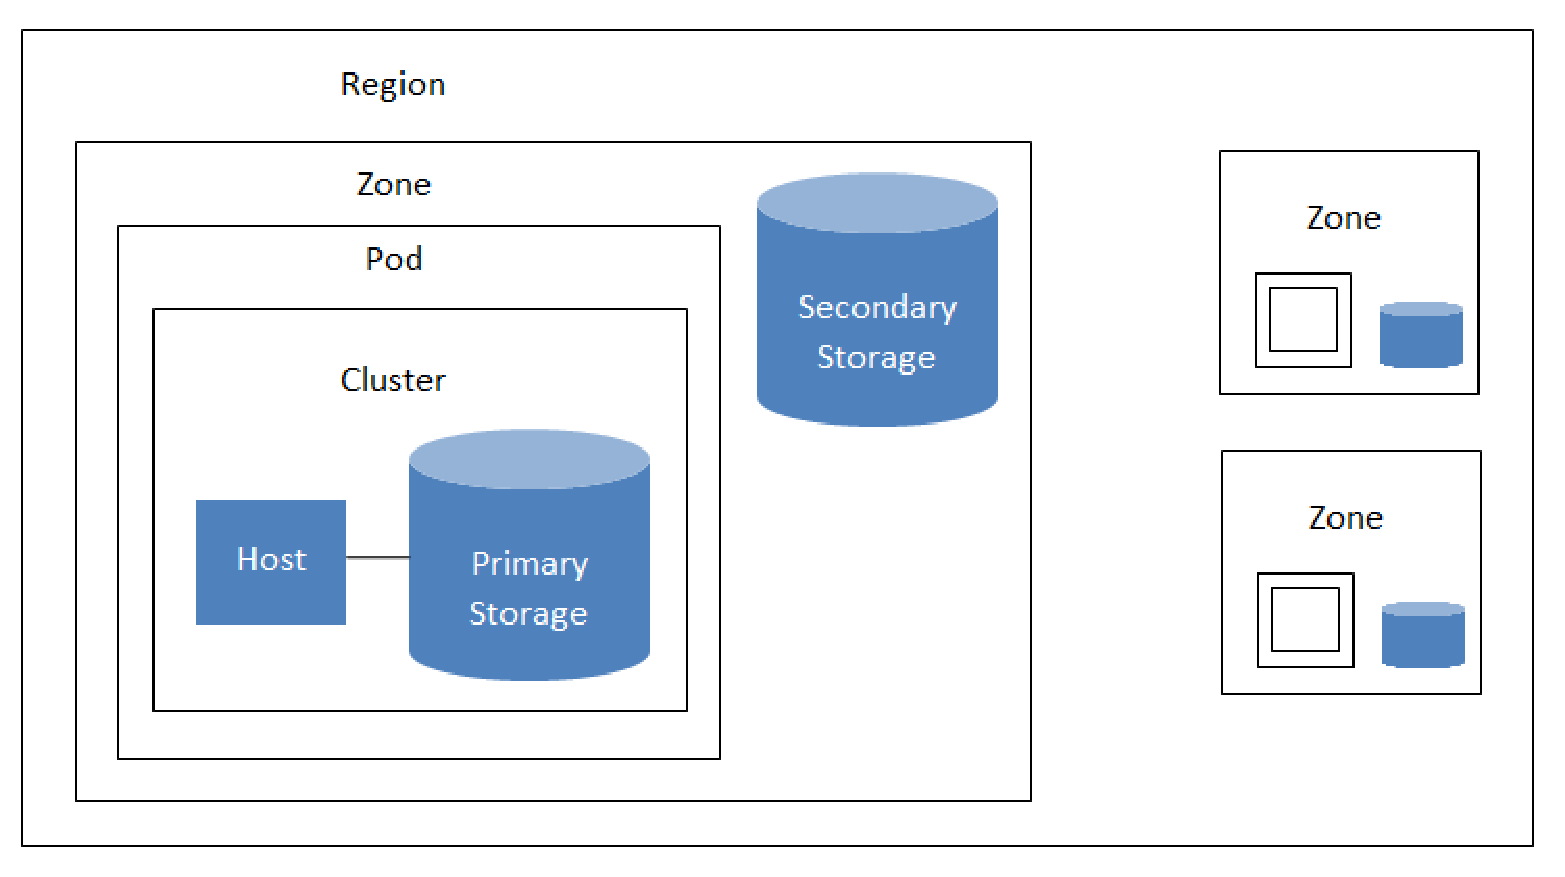
\includegraphics [keepaspectratio=true,scale=0.60]{figuras/cloudstack_structure.eps}
\caption{Visão geral da infraestrutura do Cloudstack}
\cite{cloudstack}.
\label{diagramacloudstack}
\end{figure}

